\section{A bottleneck-first taxonomy}
\label{sec:taxonomy}

Table~\ref{tab:taxonomy} organizes techniques by the bottleneck they attack. Families are complementary: weight bits do not replace KV paging; speculative decoding does not shrink the checkpoint. On everyday devices the \emph{order} is not optional.

\begin{table*}[t]
  \centering
  \small
  \caption{Taxonomy of LLM inference optimizations. ``Daily-driver rank'' is how early a solo user on a 16--24\,GB machine should reach for the family.}
  \label{tab:taxonomy}
  \begin{tabularx}{\textwidth}{@{}>{\raggedright\arraybackslash}p{2.2cm}X>{\raggedright\arraybackslash}p{2.4cm}>{\raggedright\arraybackslash}p{1.6cm}@{}}
    \toprule
    Family & Representative methods & Bottleneck & Daily rank \\
    \midrule
    Weight / activation compression & FP16/BF16, INT8/4/2, GPTQ, AWQ, SmoothQuant, QuaRot, pruning, distillation & Capacity + decode bandwidth & 1st \\
    Architecture \& size & 0.5B--9B ladder, Phi/OpenELM/MobileLLM, MoE, long-context variants & Quality vs.\ fit & 1st \\
    KV cache \& context & KV quant, GQA/MQA, PagedAttention, prefix cache, H2O, StreamingLLM, SnapKV & Capacity slope in \(T\) & 2nd \\
    Attention \& prefill & FlashAttention, chunked prefill, MInference, sparse/local attn, RoPE/YaRN & Prefill compute / IO & 3rd \\
    Decode algorithms & Speculative decoding, Medusa, EAGLE, SpecInfer, graphs & Sequential decode & 4th \\
    Compilation \& runtimes & MLX, llama.cpp, MLC, ExecuTorch, \texttt{compile}, offload, mmap & Kernel efficiency & 4th \\
    Application-level & RAG sizing, prompt cache, constrained decoding, early exit & Tokens billed / prefilled & always \\
    Batching \& scheduling & Continuous batching, SLOs, disaggregated PD & Multi-request utilization & late \\
    Parallelism & Tensor, pipeline, expert, data parallel & Multi-device fit/latency & late \\
    Adapters & LoRA / QLoRA, multi-LoRA & Extra matmuls + RAM & as needed \\
    \bottomrule
  \end{tabularx}
\end{table*}

A useful stacking order for \emph{single-stream} local inference is: (1)~choose a model that can fit; (2)~quantize weights until there is OS headroom; (3)~quantize or page KV if context grows; (4)~tune prefill and \emph{shorten the prompt} if TTFT hurts; (5)~add speculation if decode still lags and RAM remains; (6)~only then change runtime or hardware. Multi-tenant serving inverts the last steps: paging and continuous batching become mandatory before exotic decode algorithms. Figure~\ref{fig:funnel} sketches the local funnel.

\begin{figure}[t]
  \centering
  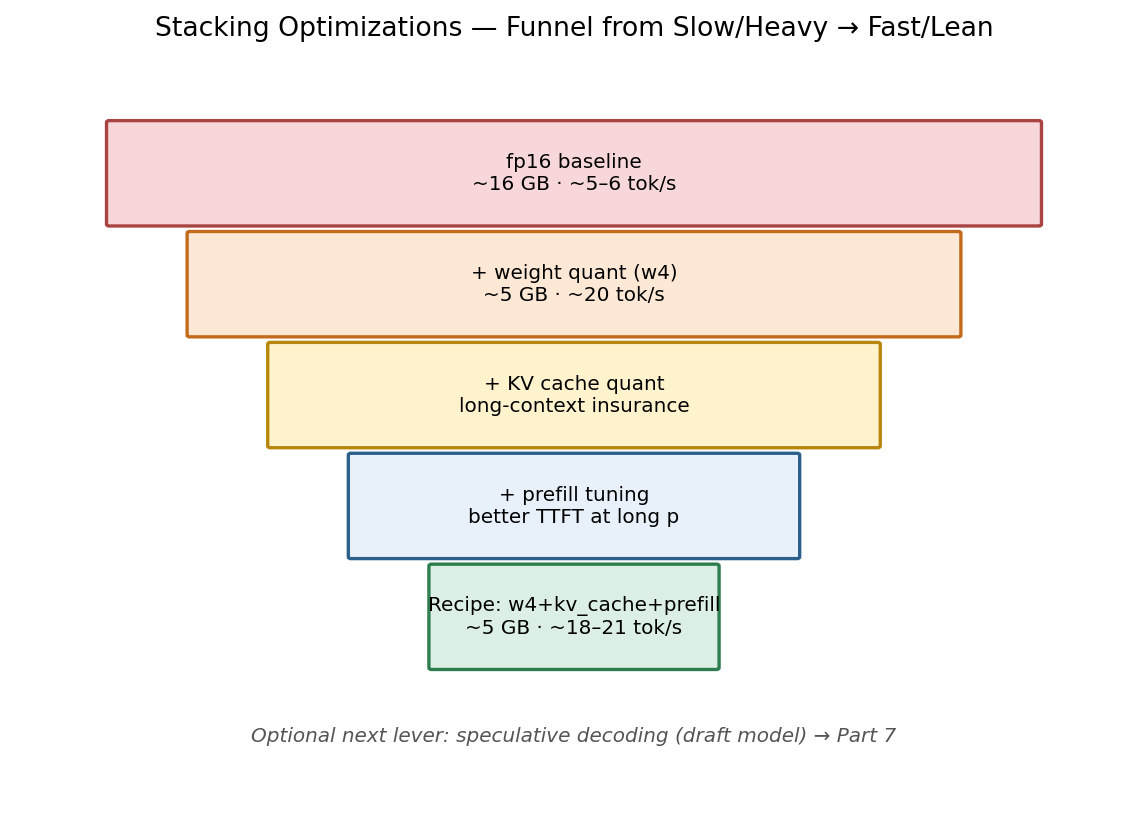
\includegraphics[width=0.98\linewidth]{figures/optimization_funnel.png}
  \caption{Local optimization funnel: weight bits shrink the floor, KV quantization insures growth in \(T\), prefill tuning attacks TTFT, and the daily recipe is the combination that survives the RAM budget \emph{with the rest of the computer still running}.}
  \label{fig:funnel}
\end{figure}
